\setcounter{tocdepth}{1} % Show chapters and sections in ToC

% Fallakte: Box am Ende jeder Station, in der die SuS ihre Erkenntnisse zum Fall Lena festhalten
\newenvironment{fallakte}[1][]
{%
	\begin{tcolorboxTemplate}[
			title=\faFolderOpen{} Fallakte Lena #1,
			parbox=false,
			colback=BurntOrange!10,
			colframe=BurntOrange!80!black,
			colbacktitle=BurntOrange!80!black]
		}%
		{%
	\end{tcolorboxTemplate}
}

% leere Schreibzeile mit vorgegebener Breite (Standard: ganze Zeile)
\newcommand{\schreibzeile}[1][\linewidth]{\par\vspace{0.6cm}\noindent\rule{#1}{0.4pt}\par}

\begin{document}

%% Project-specific Preambles
\settoggle{includelogo}{true}

\newcommand{\thesubject}{Medienkompetenzwoche}
\newcommand{\thetopic}{Datenschutz, Sicherheit \& Copyright}
\newcommand{\thelogo}{Logos/FreeFlower.pdf}
\newcommand{\logosize}{.5\textwidth}

\lhead[ \leftmark ]{\thetopic}
\rhead[\thesubject]{\textcopyleft{} \href{https://github.com/CyrilBlum/FreeFlower}{FreeFlower}, \the\year}

\settoggle{emoji}{false}
\def\arrayB{"detective","locked","camera","key","fishing-pole","copyright","check-mark-button"}
\maketitlepage{\thetopic}{Lernatelier \enquote{Der Fall Lena} -- 1.~Klassen}
\tableofcontents
\clearpage

%% content %%
\chapter{Der Fall Lena}\label{ch:fall_lena}

Lena ist 13 Jahre alt und geht in die 1.~Klasse eines Gymnasiums.
An einem Montagmorgen ist alles anders:

\begin{itemize}
	\item Auf ihrem Social-Media-Konto erscheinen Beiträge, die sie nie geschrieben hat. Ihr Passwort funktioniert nicht mehr.
	\item Ein Unbekannter schreibt ihr: \enquote{Schöner Garten übrigens. Wohnst du nicht an der Bahnhofstrasse?}
	\item Im Klassenchat macht ein Meme die Runde: ein Foto von Lena, wie sie im Schullager mit offenem Mund schläft.
\end{itemize}

\begin{figure}[H]
	\centering
	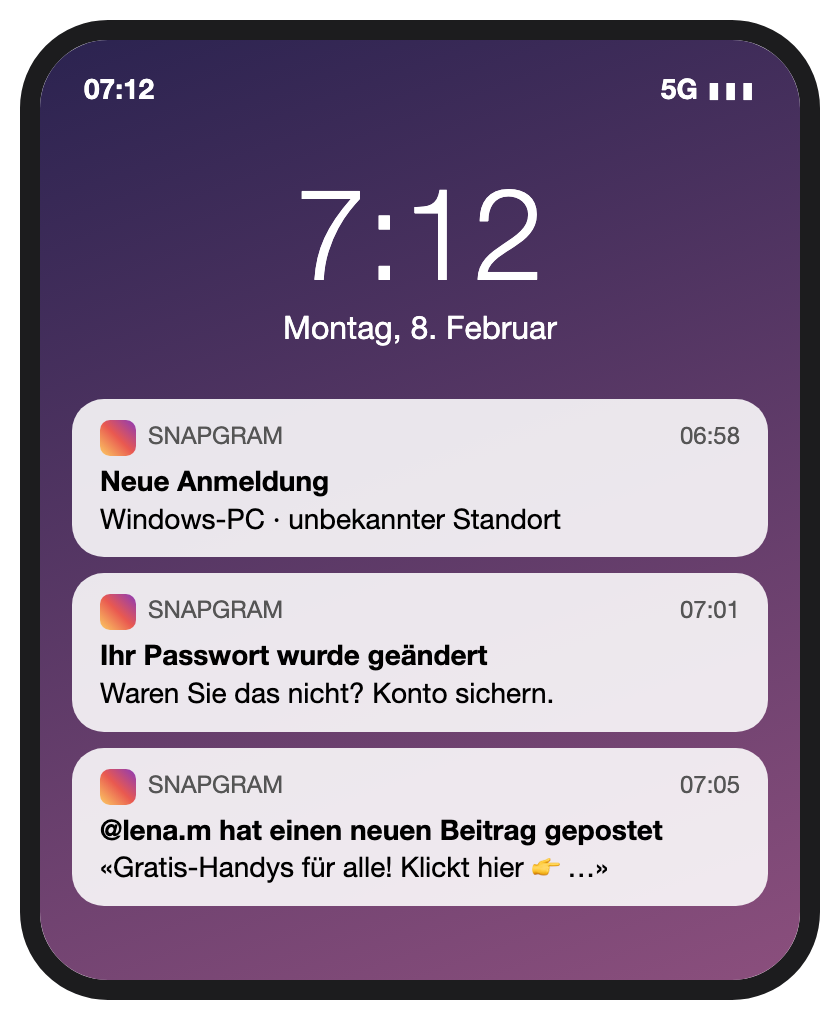
\includegraphics[height=5.6cm,keepaspectratio]{Medienkompetenzwoche/UG_Datenschutz/Figures/lena_1_gehackt}\hfill
	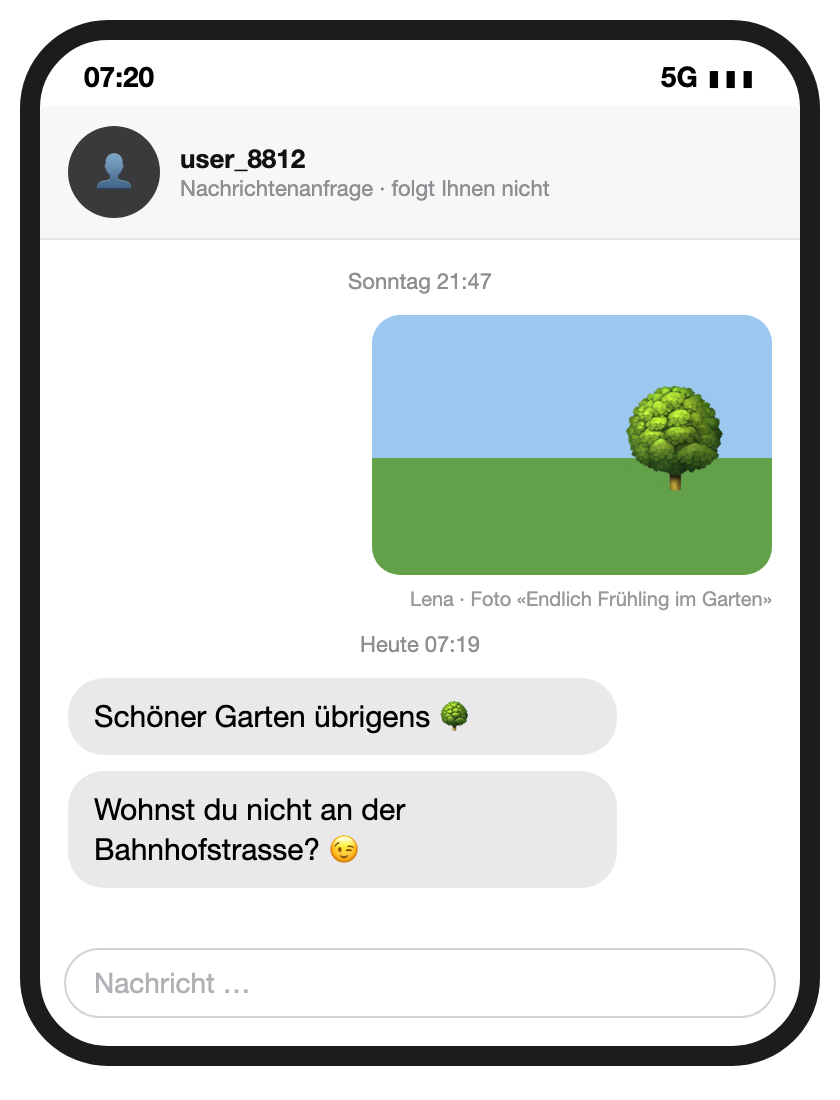
\includegraphics[height=5.6cm,keepaspectratio]{Medienkompetenzwoche/UG_Datenschutz/Figures/lena_2_nachricht}\hfill
	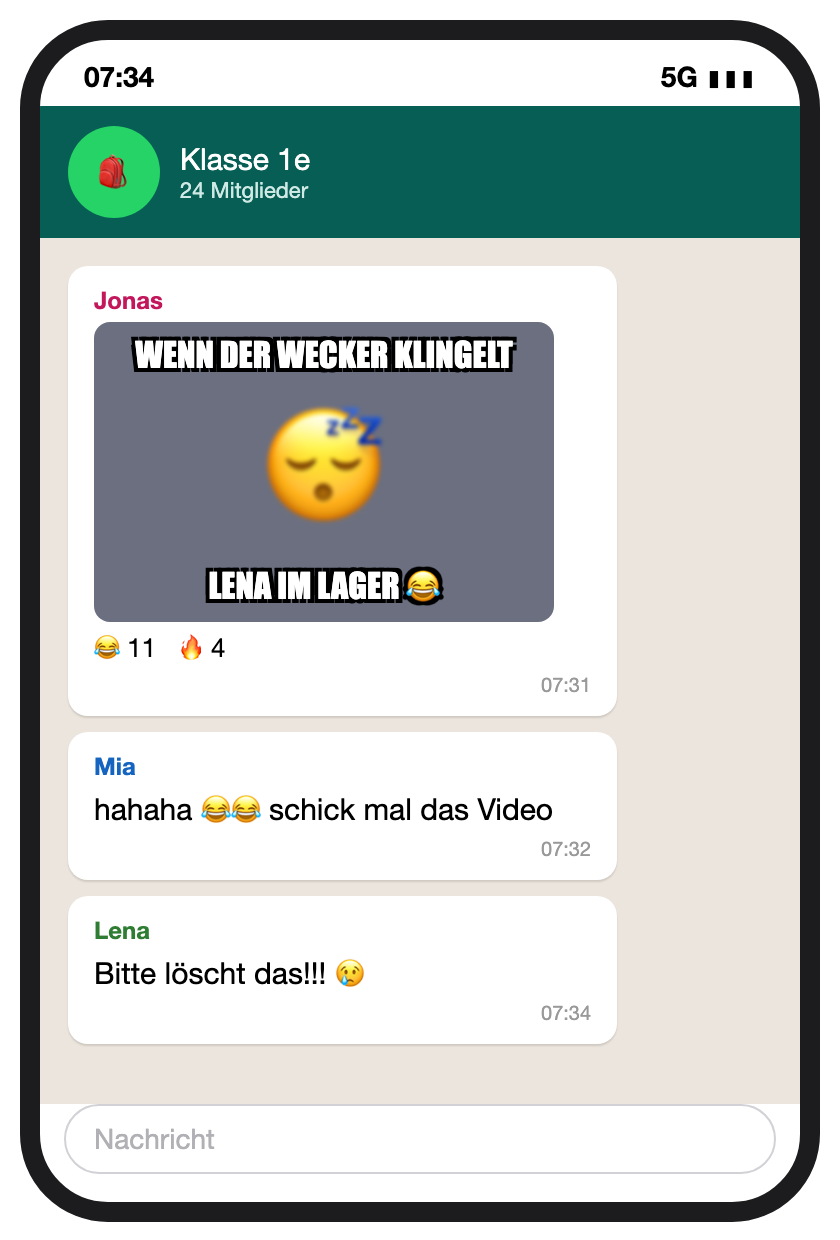
\includegraphics[height=5.6cm,keepaspectratio]{Medienkompetenzwoche/UG_Datenschutz/Figures/lena_3_klassenchat}
	\caption{Lenas Handy am Montagmorgen (nachgestellte Bildschirme, alle Namen und Dienste sind erfunden).}
	\label{fig:lena_handy}
\end{figure}

Lena versteht die Welt nicht mehr. Sie hat doch nichts Verbotenes getan -- oder doch?

\begin{myremark}
	Heute ermitteln Sie in diesem Fall. An drei Stationen finden Sie heraus,
	\textbf{wie} es dazu kommen konnte und \textbf{was} Lena (und Sie) dagegen tun können.
	Am Ende lösen Sie den Fall und erstellen ein eigenes Produkt.
\end{myremark}

\section{Ihre Lernziele}

Am Ende dieses Halbtags können Sie \dots
\begin{enumerate}
	\item erklären, welche Daten Fotos, Apps und Geräte über Sie verraten, und die wichtigsten Einstellungen auf Ihrem Handy gezielt anpassen;
	\item ein sicheres Passwort bilden, die Gefahr von wiederverwendeten Passwörtern erklären und eine Phishing-Nachricht an mindestens drei Merkmalen erkennen;
	\item an Beispielen begründet entscheiden, ob Sie ein Bild oder Video veröffentlichen dürfen, und ein frei lizenziertes Bild korrekt angeben.
\end{enumerate}

\section{So arbeiten Sie heute}

\begin{myprocedure}[Ablauf des Lernateliers]
	\begin{enumerate}
		\item \textbf{Einstieg (gemeinsam):} Die Lehrperson stellt den Fall vor und zeigt ein kurzes Experiment.
		\item \textbf{Lernatelier (zu zweit):} Sie bearbeiten die drei Stationen A, B und C in der Reihenfolge, die Ihnen die Lehrperson zuteilt. Pro Station haben Sie etwa 30--35 Minuten Zeit.
		\item \textbf{Fall lösen und Produkt (zu zweit):} Sie tragen Ihre Erkenntnisse zusammen und erstellen ein Produkt (\cref{ch:produkt}).
		\item \textbf{Abschluss (gemeinsam):} Galerie der Produkte und Auflösung des Falls.
	\end{enumerate}
\end{myprocedure}

\begin{myattention}
	\begin{itemize}
		\item Sie arbeiten teilweise mit Ihrem eigenen Handy. \textbf{Zeigen Sie niemandem private Fotos oder Nachrichten}, und schauen Sie nicht auf fremde Bildschirme.
		\item Geben Sie auf Webseiten \textbf{nie echte Passwörter} ein -- auch nicht auf Testseiten.
		\item \textbf{Pflichtaufgaben} (blau) bearbeiten alle. \textbf{Challenges} (gelb) sind für Teams, die schneller vorankommen.
		\item Wenn Sie nicht weiterkommen: zuerst im Team überlegen, dann ein anderes Team fragen, dann die Lehrperson.
	\end{itemize}
\end{myattention}

\section{Laufzettel}

Haken Sie ab, was Sie erledigt haben. So behalten Sie und die Lehrperson den Überblick.

\begin{center}
	\renewcommand{\arraystretch}{1.4}
	\begin{tabular}{lp{7.2cm}cc}
		\textbf{Station}                          & \textbf{Thema}                                & \textbf{Pflicht}       & \textbf{Challenge}     \\
		\midrule
		A (\cref{ch:spurensuche})                 & Spurensuche: Was verraten Fotos und Geräte?   & \faSquare[regular]     & \faSquare[regular]     \\
		B (\cref{ch:tatort_konto})                & Tatort Konto: Passwörter und Phishing         & \faSquare[regular]     & \faSquare[regular]     \\
		C (\cref{ch:posten})                      & Darf ich das posten?                          & \faSquare[regular]     & \faSquare[regular]     \\
		\midrule
		Fallakte (\cref{sec:fall_loesen})         & Fall Lena lösen                               & \faSquare[regular]     &                        \\
		Produkt (\cref{sec:produkt_waehlen})      & Entscheidungsbaum oder Phishing-Falle         & \faSquare[regular]     &                        \\
	\end{tabular}
\end{center}
 % Einstieg, Ablauf, Laufzettel
\chapter{Station A: Spurensuche}\label{ch:spurensuche}

\begin{myremark}
	Der Unbekannte wusste, wo Lena wohnt. Dabei hat sie ihre Adresse nie gepostet.
	Wie ist das möglich? An dieser Station finden Sie heraus, welche Spuren Fotos, Apps und Geräte hinterlassen.
\end{myremark}

\section{Was in einem Foto steckt}

Jedes Foto, das Sie mit dem Handy aufnehmen, enthält neben dem Bild selbst zusätzliche Informationen, sogenannte \tib{Metadaten}.
Sie werden im \acrshort{EXIF}-Format direkt in der Bilddatei gespeichert, zum Beispiel:
\begin{itemize}
	\item Datum und Uhrzeit der Aufnahme,
	\item Hersteller und Modell des Handys,
	\item Einstellungen der Kamera (Blitz, Belichtung, \dots),
	\item und -- falls die Standortfunktion eingeschaltet ist -- die genauen \acrshort{GPS}-Koordinaten des Aufnahmeorts.
\end{itemize}

Viele grosse Plattformen entfernen die Standortdaten beim Hochladen. Das gilt aber nicht für alle Dienste, und oft nicht, wenn ein Bild als Datei verschickt wird (z.\,B. per E-Mail, AirDrop oder \enquote{als Dokument}).
Ausserdem verrät häufig schon der Bildinhalt viel: ein Strassenschild, eine Hausnummer, das Schullogo auf dem Pullover.

\begin{myexercise}[Mein eigenes Foto]
	Öffnen Sie auf Ihrem Handy ein Foto, das Sie selbst aufgenommen haben, und lassen Sie sich die Informationen dazu anzeigen
	(iPhone: Foto antippen und nach oben wischen; Android/Google Fotos: Foto öffnen, Menü \enquote{\dots} oder nach oben wischen).
	Notieren Sie, was Sie finden. Zeigen Sie das Foto niemandem.

	\begin{center}
		\renewcommand{\arraystretch}{1.6}
		\begin{tabular}{p{5cm}p{8cm}}
			\textbf{Information}       & \textbf{Gefunden? Was steht dort?} \\
			\midrule
			Datum und Uhrzeit          &                                    \\
			Gerät (Modell)             &                                    \\
			Ort / Karte                &                                    \\
			Weitere Angaben            &                                    \\
		\end{tabular}
	\end{center}
\end{myexercise}

\begin{myexercise}[Detektivarbeit am Testfoto]\label{ex:testfoto}
	Laden Sie das Testfoto \enquote{Lena\_Garten.jpg} herunter, das Ihre Lehrperson bereitgestellt hat.
	Öffnen Sie die Dateiinformationen auf dem Laptop
	(Windows: Rechtsklick, \enquote{Eigenschaften}, Register \enquote{Details}; macOS: in \enquote{Vorschau} öffnen, \enquote{Werkzeuge}, \enquote{Informationen einblenden}).
	\begin{enumerate}
		\item Wann wurde das Foto aufgenommen?
		\item Mit welchem Gerät?
		\item Wo wurde es aufgenommen? Geben Sie die Koordinaten in eine Kartenanwendung ein.
		\item Erklären Sie in einem Satz, wie der Unbekannte Lenas Wohnort herausfinden konnte.
	\end{enumerate}
	\begin{myanswer}
		(a) 30.~Januar 2027, 14:23~Uhr. (b) Apple iPhone~13.
		(c) $47{,}35455^\circ$\,N, $8{,}55127^\circ$\,E: Chinagarten in Zürich (im Fall steht dieser Ort für Lenas Garten).
		(d) Lena hat ein Foto aus ihrem Garten verschickt, das die \acrshort{GPS}-Koordinaten enthielt. Wer die Datei erhielt, konnte den Ort auf einer Karte anzeigen.
	\end{myanswer}
\end{myexercise}

\begin{myexercise}[Standort beim Fotografieren ausschalten]
	Suchen Sie auf Ihrem Handy die Einstellung, mit der die Kamera \emph{keinen} Standort mehr speichert.
	Notieren Sie den Weg dorthin (z.\,B. \enquote{Einstellungen $\rightarrow$ \dots}).
	Entscheiden Sie selbst, ob Sie die Einstellung ändern möchten.
	\schreibzeile
	\schreibzeile
	\begin{myanswer}
		iPhone: Einstellungen $\rightarrow$ Datenschutz \& Sicherheit $\rightarrow$ Ortungsdienste $\rightarrow$ Kamera $\rightarrow$ \enquote{Nie}.
		Android: in der Kamera-App unter Einstellungen die Option \enquote{Standort speichern} bzw. \enquote{Standort-Tags} ausschalten (Bezeichnung je nach Hersteller).
		Beim Teilen auf dem iPhone kann der Ort zudem unter \enquote{Optionen} für ein einzelnes Bild entfernt werden.
	\end{myanswer}
\end{myexercise}

\section{Was Apps über Sie wissen dürfen}

Apps fragen um \tib{Berechtigungen}: Zugriff auf Standort, Kamera, Mikrofon, Kontakte oder Fotos.
Manche brauchen diese wirklich (eine Karten-App den Standort), andere sammeln damit vor allem Daten für Werbung.

\begin{myexercise}[Berechtigungs-Check]
	Wählen Sie drei Apps auf Ihrem Handy aus und prüfen Sie deren Berechtigungen
	(iPhone: Einstellungen $\rightarrow$ App auswählen; Android: Einstellungen $\rightarrow$ Apps $\rightarrow$ App $\rightarrow$ Berechtigungen).
	Tragen Sie ein, was die App darf (\faCheck) und ob sie das für ihre Aufgabe wirklich braucht.

	\begin{center}
		\renewcommand{\arraystretch}{1.6}
		\small
		\begin{tabular}{p{2.4cm}cccc p{3.2cm}}
			\textbf{App} & \textbf{Standort} & \textbf{Kamera} & \textbf{Mikrofon} & \textbf{Kontakte} & \textbf{Braucht sie das?} \\
			\midrule
			             &                   &                 &                   &                   &                           \\
			             &                   &                 &                   &                   &                           \\
			             &                   &                 &                   &                   &                           \\
		\end{tabular}
	\end{center}
\end{myexercise}

\section{Ihr Gerät hat einen Fingerabdruck}

Viele Menschen lehnen auf Webseiten die Cookies ab, damit sie nicht verfolgt werden.
Die Werbebranche nutzt deshalb zunehmend eine andere Methode: das \tib{Fingerprinting}.
Dabei liest eine Webseite Dutzende harmlose Merkmale Ihres Geräts aus -- Bildschirmgrösse, Zeitzone, Sprache, installierte Schriftarten, Version des Betriebssystems und vieles mehr.
Einzeln sagen diese Merkmale wenig aus. Zusammen ergeben sie aber eine Kombination, die je nach Messung bei 80 bis 90 Prozent aller Geräte einzigartig ist.
So kann ein Gerät wiedererkannt werden, auch ohne Cookies und ohne dass Sie es bemerken.

\begin{myexercise}[Wie einzigartig ist mein Browser?]
	Öffnen Sie auf Ihrem Laptop oder Handy die Seite \url{https://coveryourtracks.eff.org} und starten Sie den Test (\enquote{Test your browser}).
	\begin{enumerate}
		\item Hat Ihr Browser einen einzigartigen Fingerabdruck (\enquote{unique fingerprint})?
		\item Nennen Sie drei Merkmale, die der Test über Ihr Gerät herausgefunden hat.
	\end{enumerate}
	\schreibzeile
	\schreibzeile
\end{myexercise}

\begin{mychallenge}[Inkognito hilft nicht]
	Wiederholen Sie den Test in einem privaten Fenster (Inkognito-Modus).
	Erklären Sie, warum der Inkognito-Modus zwar den Verlauf und die Cookies löscht, aber kaum gegen Fingerprinting schützt.
	\schreibzeile
	\schreibzeile
	\begin{myanswer}
		Der Inkognito-Modus speichert lokal keinen Verlauf und löscht Cookies nach dem Schliessen.
		Die Merkmale des Geräts (Bildschirm, Schriftarten, Zeitzone, Betriebssystem, \dots) bleiben aber gleich und werden der Webseite weiterhin mitgeteilt.
		Darum ergibt sich derselbe oder ein sehr ähnlicher Fingerabdruck.
	\end{myanswer}
\end{mychallenge}

\begin{mychallenge}[Spurensuche im Bild]
	Nicht nur Metadaten verraten einen Ort. Suchen Sie in einem eigenen Foto, das Sie gerne posten würden, nach Hinweisen im Bildinhalt
	(Schilder, Hausnummern, Logos, Spiegelungen). Was müssten Sie abdecken oder wegschneiden?
\end{mychallenge}

\begin{fallakte}[-- Station A]
	Was ist bei Lena schiefgelaufen? Was hätte sie anders machen können?
	\schreibzeile
	\schreibzeile
	\schreibzeile
\end{fallakte}
 % Station A: Spurensuche
\chapter{Station B: Tatort Konto}\label{ch:tatort_konto}

\begin{myremark}
	Jemand hat Lenas Konto übernommen. Lena ist sicher: \enquote{Mein Passwort kennt niemand!}
	An dieser Station finden Sie heraus, wie Angreiferinnen und Angreifer trotzdem an Passwörter kommen -- und wie Sie sich schützen.
\end{myremark}

\section{Drei Wege zu fremden Passwörtern}

\begin{mysummary}
	\begin{enumerate}
		\item \textbf{Ausprobieren:} Ein Computer probiert automatisch sehr viele Passwörter durch. Zuerst bekannte Passwörter und Wörter aus dem Wörterbuch, dann alle möglichen Kombinationen.
		\item \textbf{Datenleck:} Eine Webseite wird gehackt und die Passwörter werden veröffentlicht. Wer überall dasselbe Passwort nutzt, verliert so alle Konten auf einmal.
		\item \textbf{Phishing:} Eine gefälschte Nachricht lockt auf eine gefälschte Login-Seite. Man gibt das Passwort freiwillig ein -- direkt an die Betrüger.
	\end{enumerate}
\end{mysummary}

\section{Wie lange dauert das Ausprobieren?}

Ein leistungsstarker Computer kann bei einem gestohlenen Passwortspeicher etwa \tib{10 Milliarden} ($10^{10}$) Passwörter pro Sekunde ausprobieren.
Wie viele Möglichkeiten es gibt, hängt vom \tib{Zeichenvorrat} (wie viele verschiedene Zeichen) und der \tib{Länge} ab:
Bei 26 Kleinbuchstaben und Länge 6 gibt es $26 \cdot 26 \cdot 26 \cdot 26 \cdot 26 \cdot 26 = 26^6$ Möglichkeiten.

\begin{myexercise}[Passwörter knacken -- nachgerechnet]\label{ex:passwort_rechnen}
	Ergänzen Sie die Tabelle mit dem Taschenrechner. Die erste Zeile ist als Beispiel ausgefüllt.
	Rechnen Sie die Zeit in eine anschauliche Einheit um (Sekunden, Stunden, Tage, Jahre).

	\begin{center}
		\renewcommand{\arraystretch}{1.6}
		\begin{tabular}{p{4.4cm}ccp{2.4cm}p{2.6cm}}
			\textbf{Passwort-Art}             & \textbf{Vorrat} & \textbf{Länge} & \textbf{Möglichkeiten}  & \textbf{Zeit}         \\
			\midrule
			nur Kleinbuchstaben               & 26              & 6              & $26^6 \approx \num{3.1e8}$ & \num{0.03}~s        \\
			nur Kleinbuchstaben               & 26              & 8              &                         &                       \\
			Klein-, Grossbuchstaben, Ziffern  & 62              & 8              &                         &                       \\
			Klein-, Grossbuchstaben, Ziffern  & 62              & 12             &                         &                       \\
			4 zufällige Wörter aus einer Liste & 7776           & 4              &                         &                       \\
			5 zufällige Wörter aus einer Liste & 7776           & 5              &                         &                       \\
		\end{tabular}
	\end{center}

	Was hilft mehr: ein grösserer Zeichenvorrat oder eine grössere Länge? Begründen Sie mit der Tabelle.
	\schreibzeile

	\begin{myanswer}
		\begin{tabular}{lll}
			26, Länge 8:   & $\approx \num{2.1e11}$ & ca. 21~s               \\
			62, Länge 8:   & $\approx \num{2.2e14}$ & ca. 6~Stunden           \\
			62, Länge 12:  & $\approx \num{3.2e21}$ & ca. \num{10000}~Jahre   \\
			4 Wörter:      & $\approx \num{3.7e15}$ & ca. 4~Tage              \\
			5 Wörter:      & $\approx \num{2.8e19}$ & ca. 90~Jahre            \\
		\end{tabular}

		Die Länge hilft am meisten, weil sie im Exponenten steht: Jedes zusätzliche Zeichen vervielfacht die Anzahl Möglichkeiten.
		Wichtig: Diese Zeiten gelten nur für \emph{zufällige} Passwörter. Bekannte Wörter, Namen oder Muster wie \enquote{Hund2024!} werden mit Wörterlisten fast sofort gefunden.
	\end{myanswer}
\end{myexercise}

\section{Ein gutes Passwort bauen}

\begin{myprocedure}[Zwei Methoden für starke Passwörter]
	\begin{itemize}
		\item \textbf{Wörter-Methode:} Wählen Sie vier oder fünf \emph{zufällige} Wörter, die nichts miteinander zu tun haben, z.\,B. \enquote{Kaktus Wolke Trompete Senf Igel}.
		      Lang, aber gut zu merken.
		\item \textbf{Satz-Methode:} Denken Sie sich einen Satz aus und nehmen Sie die Anfangsbuchstaben, Zahlen und Satzzeichen:
		      \enquote{Am Montag esse ich 2 Gipfeli und trinke 1 Kakao!} wird zu \enquote{AMei2Gut1K!}.
	\end{itemize}
	Für jedes Konto ein anderes Passwort -- dabei hilft ein \tib{Passwortmanager}, der alle Passwörter sicher speichert.
\end{myprocedure}

\begin{myexercise}[Passwort-Test]
	\begin{enumerate}
		\item Bilden Sie mit jeder Methode ein \emph{Beispiel}-Passwort, das Sie nirgends verwenden.
		\item Testen Sie Ihre Beispiele und zum Vergleich \enquote{Lena2013} auf der Seite\\
		      \url{https://www.passwortcheck.ch} (ein Angebot der Daten\-schutz\-beauf\-trag\-ten des Kantons Zürich). Notieren Sie die Ergebnisse.
	\end{enumerate}
	\schreibzeile
	\schreibzeile
\end{myexercise}

\begin{myexercise}[Lenas Fehler]
	Lena hatte für ihr Social-Media-Konto dasselbe Passwort wie für ein Gaming-Forum.
	Letzten Monat wurde dieses Forum gehackt und die Liste der Benutzernamen und Passwörter im Internet veröffentlicht.
	Erklären Sie, wie die Angreifer so an Lenas Social-Media-Konto kamen, und nennen Sie zwei Massnahmen, die das verhindert hätten.
	\schreibzeile
	\schreibzeile
	\schreibzeile
	\begin{myanswer}
		Angreifer probieren veröffentlichte Kombinationen aus Benutzername (oder E-Mail) und Passwort automatisch bei anderen Diensten aus.
		Weil Lena das Passwort wiederverwendet hat, funktionierte es auch bei ihrem Social-Media-Konto.
		Massnahmen: für jedes Konto ein eigenes Passwort (Passwortmanager); \gls{TFA} einschalten.
	\end{myanswer}
\end{myexercise}

\section{Der zweite Schlüssel}

Bei der \tib{Zwei-Faktor-Authentifizierung} (\acrshort{TFA}) braucht es für die Anmeldung zwei verschiedene Dinge:
etwas, das Sie \emph{wissen} (Passwort), und etwas, das Sie \emph{haben} (Handy mit Code-App oder SMS-Code).
Selbst wer Ihr Passwort kennt, kommt ohne Ihr Handy nicht in Ihr Konto.

\begin{myexercise}[Habe ich einen zweiten Schlüssel?]
	Finden Sie bei einer App oder einem Konto, das Sie nutzen, die Einstellung für die \gls{TFA}
	(oft unter \enquote{Sicherheit}, \enquote{Anmeldung} oder \enquote{Konto}). Ist sie eingeschaltet?
	Notieren Sie den Weg. Aktivieren Sie sie, wenn Sie möchten -- bei Unsicherheit zusammen mit Ihren Eltern.
	\schreibzeile
\end{myexercise}

\section{Phishing-Detektiv}

Phishing-Nachrichten wirken oft echt. Seit es \gls{KI} gibt, sind sie sogar fehlerfrei und persönlich formuliert.
Achten Sie deshalb weniger auf Rechtschreibfehler, sondern auf diese \tib{Warnsignale}:
Zeitdruck oder Drohung, ungewöhnliche Bitte (Geld, Passwort, Code), unbekannter Absender, Link mit seltsamer Adresse, \enquote{zu gut, um wahr zu sein}.

\begin{myexercise}[Echt oder Falle?]\label{ex:phishing}
	Entscheiden Sie bei jeder Nachricht: echt oder Falle? Notieren Sie die Warnsignale in der Tabelle. Alle Firmen, Adressen und Nummern sind erfunden.

	\begin{center}
		\begin{tabular}{ccc}
			\textbf{(a)} SMS & \textbf{(b)} Mitteilung & \textbf{(c)} Chat \\
			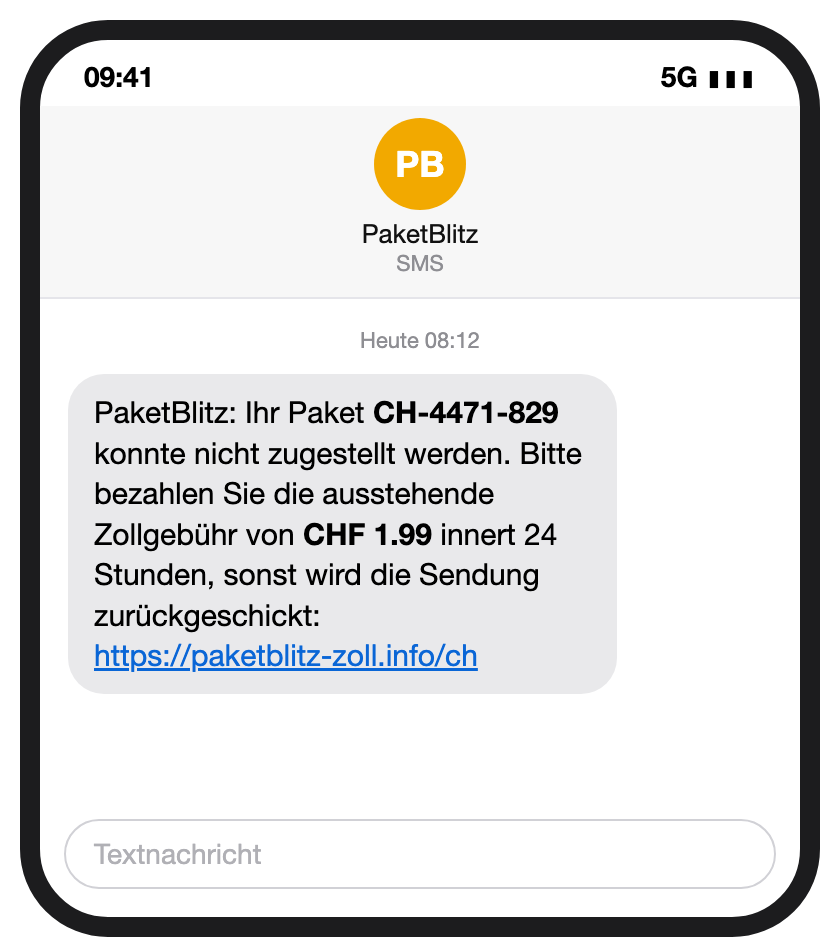
\includegraphics[height=5.4cm,keepaspectratio]{Medienkompetenzwoche/UG_Datenschutz/Figures/1_sms_paketblitz} &
			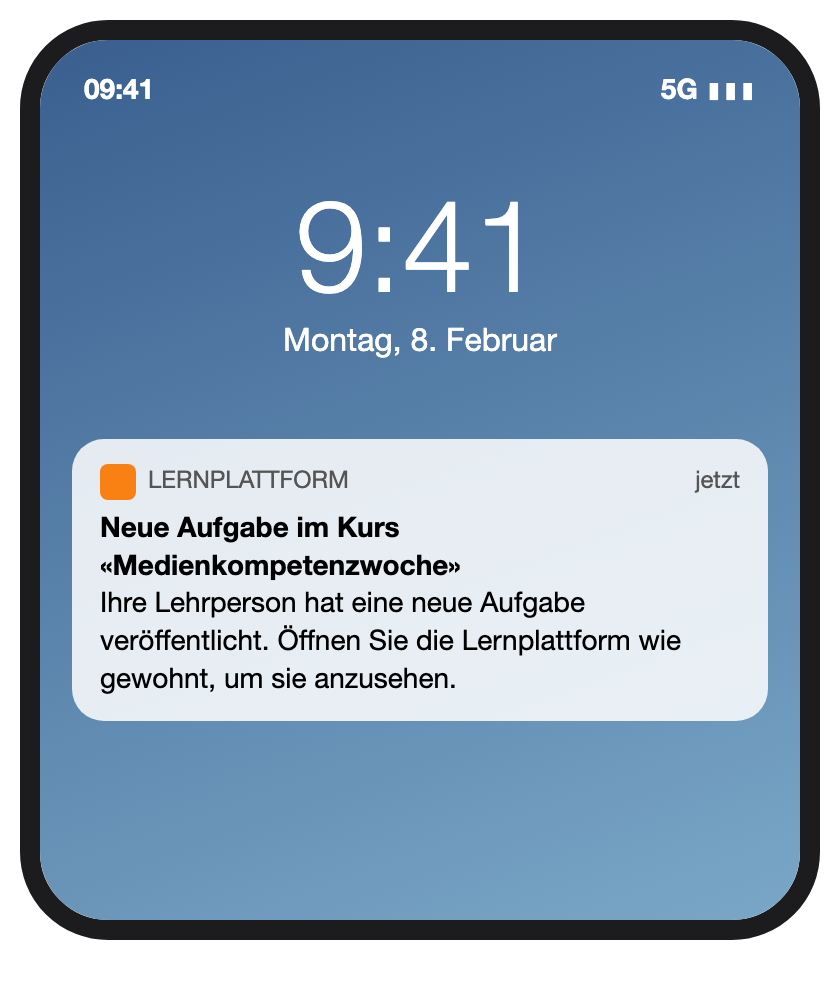
\includegraphics[height=5.4cm,keepaspectratio]{Medienkompetenzwoche/UG_Datenschutz/Figures/3_push_lernplattform} &
			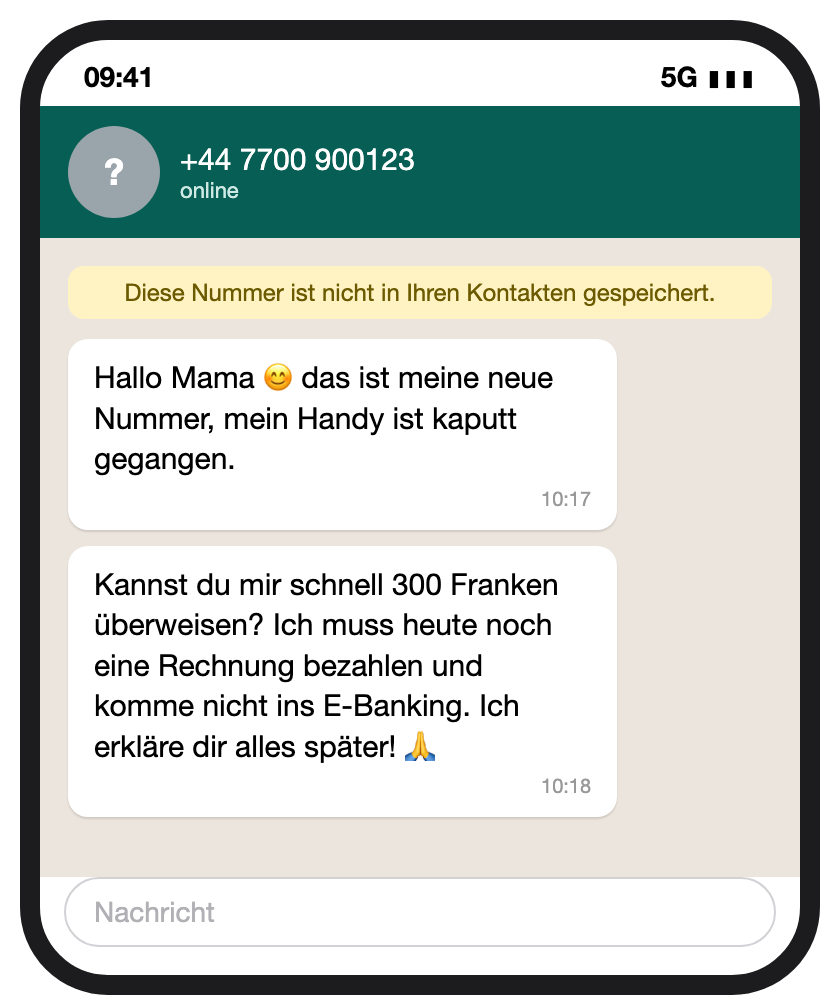
\includegraphics[height=5.4cm,keepaspectratio]{Medienkompetenzwoche/UG_Datenschutz/Figures/4_chat_hallomama} \\[3mm]
		\end{tabular}

		\textbf{(d)} E-Mail\\[1mm]
		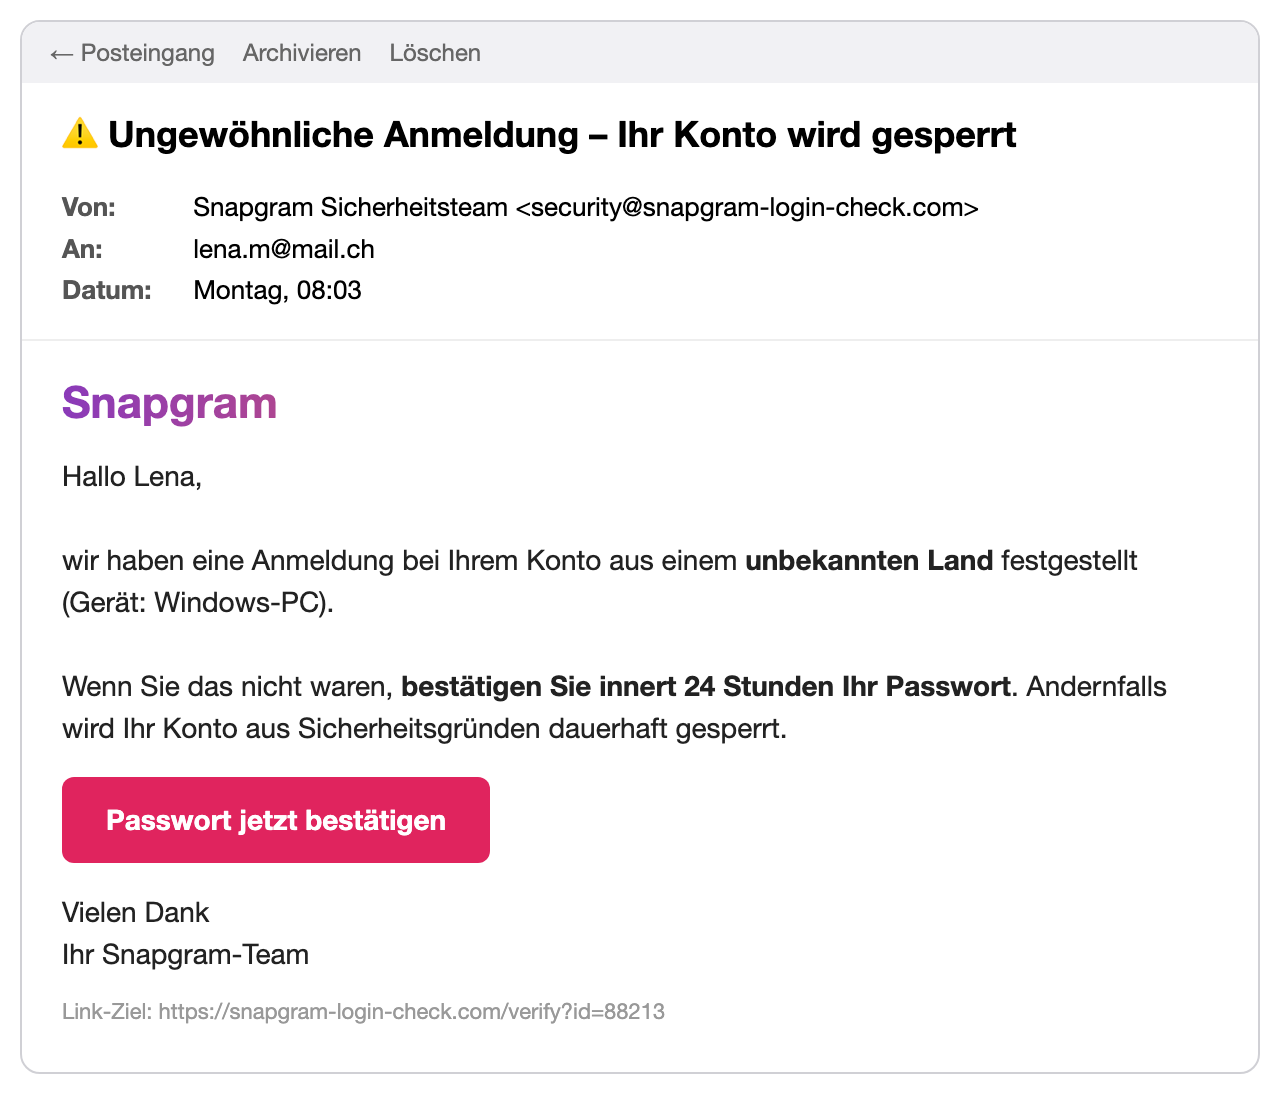
\includegraphics[width=0.72\linewidth,keepaspectratio]{Medienkompetenzwoche/UG_Datenschutz/Figures/2_mail_snapgram}
	\end{center}

	\begin{center}
		\renewcommand{\arraystretch}{1.5}
		\begin{tabular}{p{0.8cm}p{2.6cm}p{9cm}}
			\textbf{Nr.} & \textbf{echt / Falle} & \textbf{Warnsignale}  \\
			\midrule
			(a)          &                       &                       \\
			(b)          &                       &                       \\
			(c)          &                       &                       \\
			(d)          &                       &                       \\
		\end{tabular}
	\end{center}

	\begin{myanswer}
		\begin{aenum}
			\item Falle: Zeitdruck, kleiner Betrag als Köder (es geht um die Kreditkartendaten), fremde Internetadresse.
			\item Wahrscheinlich echt: kein Link, keine Bitte um Daten, man soll die Plattform \enquote{wie gewohnt} öffnen. Trotzdem gilt: nie über Links in Nachrichten anmelden.
			\item Falle (\enquote{Hallo-Mama}-Betrug): unbekannte (ausländische) Nummer, Geldforderung, Zeitdruck. Immer über die bekannte Nummer zurückrufen.
			\item Falle: Drohung (Sperrung), Zeitdruck, Aufforderung zur Passworteingabe; die Adressen von Absender und Link gehören nicht zum echten Dienst.
		\end{aenum}
	\end{myanswer}
\end{myexercise}

\begin{mychallenge}[Phishing-Quiz]
	Machen Sie das Phishing-Quiz unter \url{https://phishingquiz.withgoogle.com}. Name und E-Mail-Adresse dürfen Sie erfinden.
	Wie viele von acht Nachrichten haben Sie richtig erkannt? Welches Warnsignal hatten Sie übersehen?
	\schreibzeile
\end{mychallenge}

\begin{fallakte}[-- Station B]
	Wie kamen die Angreifer an Lenas Konto? Was hätte sie anders machen können?
	\schreibzeile
	\schreibzeile
	\schreibzeile
\end{fallakte}
 % Station B: Tatort Konto
\chapter{Station C: Darf ich das posten?}\label{ch:posten}

\begin{myremark}
	Das Meme von der schlafenden Lena finden viele lustig -- Lena nicht.
	Durfte das überhaupt jemand posten? An dieser Station lernen Sie die wichtigsten Regeln für Bilder, Videos und Musik kennen.
\end{myremark}

\section{Zwei Rechte, die Sie kennen müssen}

\begin{mysummary}[Urheberrecht]
	Wer etwas erschafft -- ein Foto, eine Zeichnung, einen Text, ein Lied --, ist \tib{Urheberin} oder \tib{Urheber} und entscheidet, ob und wie das Werk veröffentlicht wird.
	Geregelt ist das im \gls{URG}.
	\begin{itemize}
		\item In der Schweiz ist seit 2020 \textbf{jedes Foto} geschützt, auch ein einfacher Schnappschuss.
		\item Im \textbf{privaten Kreis} (Familie, enge Freunde) dürfen Sie Werke nutzen und teilen.
		      Öffentlich posten gehört \emph{nicht} mehr zum privaten Kreis.
		\item Ein Bild aus der Internetsuche ist darum \emph{nicht} automatisch frei verwendbar.
	\end{itemize}
\end{mysummary}

\begin{mysummary}[Recht am eigenen Bild]
	Jede Person darf grundsätzlich selbst bestimmen, ob Bilder von ihr veröffentlicht werden.
	Das folgt aus dem Persönlichkeitsschutz im \gls{ZGB}.
	\begin{itemize}
		\item Wer auf einem Bild \textbf{erkennbar} ist und im Mittelpunkt steht, muss in der Regel \textbf{einverstanden} sein.
		\item Bei einer grossen Menschenmenge (Konzert, Sportanlass) ist das meist nicht nötig, solange niemand gezielt herausgehoben wird.
		\item Blossstellende oder verletzende Bilder sind besonders heikel -- sie können Cybermobbing sein.
	\end{itemize}
\end{mysummary}

\begin{myexercise}[Fallkarten: Darf ich das posten?]\label{ex:fallkarten}
	Entscheiden Sie zu zweit: \faCheck{} erlaubt, \faTimes{} nicht erlaubt oder \textbf{?} kommt darauf an. Begründen Sie kurz.

	\begin{center}
		\renewcommand{\arraystretch}{1.5}
		\small
		\begin{tabular}{p{0.6cm}p{7.4cm}cp{3.8cm}}
			\textbf{Nr.} & \textbf{Situation}                                                                                        & \textbf{\faCheck/\faTimes/?} & \textbf{Begründung} \\
			\midrule
			1            & Ein Selfie, auf dem nur Sie zu sehen sind, als Profilbild.                                                &                              &                     \\
			2            & Ein Gruppenfoto der Klasse auf Ihrem öffentlichen Profil, ohne die anderen zu fragen.                       &                              &                     \\
			3            & Das Foto der schlafenden Lena als Meme im Klassenchat.                                                    &                              &                     \\
			4            & Ein Bild aus der Internet-Bildersuche als Titelbild für Ihren Blog.                                       &                              &                     \\
			5            & Ein Bild von Wikimedia Commons mit der Lizenz \gls{CC}~BY auf einem Schulplakat, mit Angabe der Urheberin. &                              &                     \\
			6            & Ihr Lieblingssong als Hintergrundmusik in einem eigenen Kurzvideo.                                        &                              &                     \\
			7            & Ein Foto vom Konzert mit Tausenden Zuschauenden.                                                          &                              &                     \\
			8            & Ein Screenshot aus einem privaten Chat mit einer Kollegin in Ihrer Story.                                 &                              &                     \\
		\end{tabular}
	\end{center}

	\begin{myanswer}
		\begin{enumerate}
			\item \faCheck{} Sie sind Urheber und abgebildete Person zugleich.
			\item \faTimes{} Alle erkennbaren Personen müssen einverstanden sein.
			\item \faTimes{} Verletzt Lenas Recht am eigenen Bild und ist blossstellend (Cybermobbing). Auch ein Klassenchat ist nicht mehr nur der enge private Kreis.
			\item \faTimes{} Bilder aus der Suche sind in der Regel urheberrechtlich geschützt. Lizenz prüfen oder freie Bilder suchen.
			\item \faCheck{} Die Lizenz erlaubt die Nutzung, wenn die Urheberin korrekt genannt wird.
			\item \textbf{?} Kommt auf die Plattform an: Manche haben Lizenzen für ihre eigene Musikbibliothek. Einen Song selbst hochzuladen und öffentlich zu verwenden, ist ohne Erlaubnis nicht zulässig.
			\item \faCheck{} Menschenmenge, niemand steht im Mittelpunkt. Das Foto haben Sie selbst gemacht.
			\item \faTimes{} Private Nachrichten sind vertraulich; die Kollegin muss einverstanden sein.
		\end{enumerate}
	\end{myanswer}
\end{myexercise}

\section{Freie Bilder finden und richtig angeben}

Mit einer \tib{Creative-Commons-Lizenz} (\gls{CC}) erlauben Urheberinnen und Urheber allen, ihr Werk unter bestimmten Bedingungen zu nutzen:

\begin{center}
	\renewcommand{\arraystretch}{1.3}
	\begin{tabular}{lp{11cm}}
		\textbf{Kürzel} & \textbf{Bedeutung}                                                                 \\
		\midrule
		BY              & Namensnennung: Die Urheberin oder der Urheber muss genannt werden.                 \\
		SA              & Weitergabe unter gleichen Bedingungen: Veränderte Werke brauchen dieselbe Lizenz.  \\
		NC              & Nicht kommerziell: keine Nutzung, mit der Geld verdient wird.                      \\
		ND              & Keine Bearbeitung: Das Werk darf nicht verändert werden.                           \\
		CC0             & Kein Vorbehalt: frei nutzbar, Namensnennung freiwillig.                            \\
	\end{tabular}
\end{center}

Für eine korrekte Angabe hilft die Regel \tib{TULLU}: \textbf{T}itel, \textbf{U}rheber/in, \textbf{L}izenz, \textbf{L}ink zur Lizenz, \textbf{U}rsprungsort.

\begin{myexample}
	\enquote{Rotkehlchen im Schnee} von Max Muster, Lizenz CC~BY~4.0 (\url{https://creativecommons.org/licenses/by/4.0/}), Quelle: Wikimedia Commons.
\end{myexample}

\begin{myexercise}[Ein freies Bild für Lena]
	Lena möchte ein neues Profilbild ohne ihr Gesicht, zum Beispiel ein Tier oder eine Landschaft.
	Suchen Sie auf \url{https://openverse.org} oder \url{https://commons.wikimedia.org} ein passendes Bild mit einer \gls{CC}-Lizenz
	und schreiben Sie die vollständige Angabe nach TULLU auf.
	\schreibzeile
	\schreibzeile
\end{myexercise}

\begin{mychallenge}[Unter welcher Lizenz steht dieses Skript?]
	Finden Sie auf dem Titelblatt oder in der Kopfzeile heraus, unter welcher Lizenz dieses Skript steht
	(Tipp: Folgen Sie dem Link zu FreeFlower). Erklären Sie, was Sie damit tun dürfen und was nicht.
	\schreibzeile
	\schreibzeile
	\begin{myanswer}
		Das Skript steht unter \gls{CC}~BY-NC-SA~4.0: Man darf es kopieren, weitergeben und verändern,
		muss die Urheber nennen, darf damit kein Geld verdienen und muss veränderte Fassungen unter derselben Lizenz weitergeben.
	\end{myanswer}
\end{mychallenge}

\begin{mychallenge}[Und KI-Bilder?]
	Mit \gls{KI} lassen sich Bilder in Sekunden erzeugen. Diskutieren Sie zu zweit: Wem gehört ein solches Bild?
	Darf man ein KI-Bild einer echten Person posten, das diese Person nie so gesehen hat?
	Halten Sie Ihre wichtigsten Argumente fest. (Hinweis: Die Rechtslage ist noch nicht in allen Punkten geklärt. Klar ist aber, dass das Recht am eigenen Bild auch hier gilt.)
	\schreibzeile
	\schreibzeile
\end{mychallenge}

\begin{fallakte}[-- Station C]
	Durfte das Meme von Lena gepostet werden? Was kann Lena jetzt tun?
	\schreibzeile
	\schreibzeile
	\schreibzeile
	\begin{myanswer}
		Nein, Lena war erkennbar und nicht einverstanden; das Bild stellt sie bloss.
		Lena kann die Person bitten, das Bild zu löschen, es der Plattform bzw. im Chat melden, Screenshots als Beweis sichern
		und sich an eine Vertrauensperson (Eltern, Klassenlehrperson) wenden. Beratung bietet z.\,B. Pro Juventute (Telefon 147).
	\end{myanswer}
\end{fallakte}
 % Station C: Darf ich das posten?
\chapter{Fall lösen und Produkt}\label{ch:produkt}

\section{Den Fall Lena lösen}\label{sec:fall_loesen}

\begin{myexercise}[Die Auflösung]
	Tragen Sie Ihre drei Fallakten zusammen. Schreiben Sie Lena eine kurze Nachricht (4--6 Sätze):
	Was ist passiert, und welche \textbf{drei} Dinge sollte sie ab heute anders machen?
	\schreibzeile
	\schreibzeile
	\schreibzeile
	\schreibzeile
	\schreibzeile
	\begin{myanswer}
		Mögliche Punkte: Standort in der Kamera ausschalten bzw. Fotos ohne Ortsangaben verschicken;
		für jedes Konto ein eigenes, langes Passwort verwenden und die \gls{TFA} einschalten;
		bei Nachrichten mit Zeitdruck oder Passwortabfrage nie auf Links klicken;
		bei blossstellenden Bildern die Löschung verlangen, melden und Hilfe holen.
	\end{myanswer}
\end{myexercise}

\section{Ihr Produkt}\label{sec:produkt_waehlen}

Wählen Sie im Team \textbf{eines} der beiden Produkte. Zeit: etwa 30 Minuten.

\subsection{Produkt 1: Entscheidungsbaum \enquote{Darf ich das posten?}}

Gestalten Sie auf einem A3-Plakat einen Entscheidungsbaum, mit dem eine Mitschülerin in wenigen Sekunden prüfen kann, ob sie ein Bild oder Video posten darf.
Der folgende Anfang zeigt die Idee. Ergänzen Sie mindestens drei weitere Fragen (z.\,B. zu Lizenzen, Musik, Standort im Bild) und gestalten Sie das Plakat ansprechend.

\begin{center}
	\begin{tikzpicture}[
			node distance=0.9cm and 1.4cm,
			frage/.style={draw=RoyalBlue, fill=RoyalBlue!10, rounded corners, align=center, text width=4.2cm, minimum height=1cm},
			ja/.style={draw=ForestGreen, fill=ForestGreen!10, rounded corners, align=center, text width=3cm},
			nein/.style={draw=BrickRed, fill=BrickRed!10, rounded corners, align=center, text width=3cm},
			pfeil/.style={-{Stealth}, thick},
			lbl/.style={font=\small, fill=white, inner sep=1pt}
		]
		\node[frage] (f1) {Habe ich das Bild selbst gemacht?};
		\node[frage, below=of f1] (f2) {Sind Personen erkennbar?};
		\node[nein, right=of f1] (n1) {Lizenz prüfen \\ (\cref{ex:fallkarten}, Nr.~4 und 5)};
		\node[frage, below=of f2] (f3) {Sind alle einverstanden?};
		\node[ja, left=of f2] (j1) {\dots weitere Fragen \dots};
		\node[nein, right=of f3] (n2) {Nicht posten!};
		\node[ja, below=of f3] (j2) {\dots weitere Fragen \dots};

		\draw[pfeil] (f1) -- node[lbl] {nein} (n1);
		\draw[pfeil] (f1) -- node[lbl] {ja} (f2);
		\draw[pfeil] (f2) -- node[lbl] {nein} (j1);
		\draw[pfeil] (f2) -- node[lbl] {ja} (f3);
		\draw[pfeil] (f3) -- node[lbl] {nein} (n2);
		\draw[pfeil] (f3) -- node[lbl] {ja} (j2);
	\end{tikzpicture}
\end{center}

\subsection{Produkt 2: Phishing-Falle bauen}

Gestalten Sie auf einer Karte eine erfundene Phishing-Nachricht (SMS, E-Mail oder Chat), die möglichst echt wirkt und \textbf{mindestens drei} Warnsignale versteckt.
Notieren Sie die Lösung auf der Rückseite. Danach tauschen Sie die Karte mit einem anderen Team: Wer findet alle Warnsignale?

\begin{myattention}
	Verwenden Sie nur \textbf{erfundene} Firmen, Namen und Adressen. Keine echten Links, keine echten Personen, keine echten Logos.
\end{myattention}

\subsection{Checkliste für Ihr Produkt}

\begin{center}
	\renewcommand{\arraystretch}{1.4}
	\begin{tabular}{p{12.5cm}c}
		\textbf{Kriterium}                                                                   & \textbf{erfüllt}   \\
		\midrule
		Der Inhalt ist fachlich richtig (vergleichen Sie mit den Stationen A--C).            & \faSquare[regular] \\
		Das Produkt ist ohne Erklärung verständlich.                                         & \faSquare[regular] \\
		Es enthält mindestens drei eigene Ideen (Fragen bzw. Warnsignale).                   & \faSquare[regular] \\
		Es verletzt selbst keine Rechte (keine fremden Bilder ohne Lizenz, keine echten Personen). & \faSquare[regular] \\
	\end{tabular}
\end{center}

\section{Exit-Ticket}

\begin{myexercise}[Eine Sache ändere ich heute noch]
	Notieren Sie \textbf{eine} konkrete Sache, die Sie heute noch an Ihrem Handy oder Ihren Konten ändern werden.
	\schreibzeile
\end{myexercise}
 % Fall lösen und Produkt

\clearpage
\appendix
\chapter{Hinweise für Lehrpersonen}\label{app:lehrpersonen}

\begin{myremark}
	Entwurf vom 24.10.2026 zur Diskussion im Team Modul~B (Cyril Blum, Stephan Pestalozzi).
	Modul~B läuft am Montag zweimal (Morgen: U1c/U1d, Nachmittag: U1a/U1b) mit je zwei parallelen Gruppen;
	beide Lehrpersonen arbeiten mit demselben Ablauf.
\end{myremark}

\section{Konzept}

Der Halbtag ist als \tib{Lernatelier} mit einer durchgehenden Fallgeschichte aufgebaut.
Rund zwei Drittel der Zeit arbeiten die SuS selbstständig in Zweierteams an drei Stationen.
Jede Station schliesst mit einem Eintrag in die \enquote{Fallakte}; am Schluss wird der Fall gelöst und ein kleines Produkt erstellt.
Pflichtaufgaben sichern die Lernziele, Challenges differenzieren nach oben.
Die Lehrperson begleitet, gibt Tipps und beobachtet den Laufzettel.

\section{Ablauf (ca. 180 Minuten netto)}

\begin{center}
	\renewcommand{\arraystretch}{1.35}
	\begin{tabular}{p{1.9cm}p{3.4cm}p{6.4cm}p{2.4cm}}
		\textbf{Zeit}  & \textbf{Phase}           & \textbf{Inhalt}                                                                                                                    & \textbf{Sozialform} \\
		\midrule
		0--20'         & Einstieg                 & Fall Lena vorstellen; Live-Demo Fingerprinting (Cover Your Tracks am Beamer); Ablauf, Regeln, Laufzettel; Zweierteams bilden.       & Plenum              \\
		20--130'       & Lernatelier              & Stationen A, B, C à ca.\ 30--35', gestaffelter Start (je ein Drittel der Teams pro Station); Pause einbauen.                          & Zweierteams         \\
		130--165'      & Fall lösen, Produkt      & Fallakten zusammentragen, Nachricht an Lena; Produkt 1 (Entscheidungsbaum) oder 2 (Phishing-Falle); Phishing-Karten tauschen.       & Zweierteams         \\
		165--180'      & Abschluss                & Kurze Galerie, Auflösung des Falls im Plenum, Exit-Ticket.                                                                          & Plenum              \\
	\end{tabular}
\end{center}

Die Zeiten an die effektiven Lektionen und Pausen des Montags anpassen.

\section{Vorbereitung}

\begin{itemize}
	\item SuS vorab informieren: Handy und Laptop mitbringen, Akku geladen.
	\item Testfoto \enquote{Lena\_Garten.jpg} (gezeichneter Garten mit \acrshort{EXIF}-Daten: Apple iPhone~13, Aufnahme am 30.~Januar 2027 um 14:23, \acrshort{GPS} des öffentlichen Chinagartens Zürich) auf der Lernplattform bereitstellen. Vorher prüfen, ob die Plattform die Metadaten beim Hochladen entfernt; sonst als ZIP-Datei anbieten (\cref{ex:testfoto}).
	\item Erreichbarkeit der Webseiten im Schulnetz testen: coveryourtracks.eff.org, passwortcheck.ch, phishingquiz.withgoogle.com, openverse.org, commons.wikimedia.org.
	\item Material: Skript (ohne Lösungen, Klassenoption \texttt{exerciseonly}), A3-Plakate, Stifte, Karten für Produkt~2, Taschenrechner.
	\item Optional: Tippkarten pro Station (z.\,B. Wege zu den Einstellungen auf iPhone/Android).
	\item Optional: Stationen zusätzlich als Moodle-Kurs mit Selbsttests anbieten (moodle-one).
\end{itemize}

\section{Abgrenzung zu anderen Modulen}

\begin{itemize}
	\item \textbf{Zischtig.ch:} Privatsphäre-Einstellungen in Social-Media-Apps, Sexting, Hassrede, Sucht -- hier bewusst nicht vertieft.
	\item \textbf{Modul~A (digitale Achtsamkeit):} Leitfaden zur eigenen Mediennutzung; deshalb hier andere Produkte.
	\item \textbf{Modul~C (Mechanismen und Beeinflussung):} Deepfakes, Fake-Profile, Bots -- Station~C behandelt nur die Rechtsfragen.
	\item \textbf{Fach Informatik:} Verschlüsselung und Netzwerksicherheit (Kryptologie) -- hier nur Passwörter und \gls{TFA} auf Anwendungsebene.
\end{itemize}

\section{Lehrplanbezug}

\begin{itemize}
	\item Lehrplan~21, Medien und Informatik: \enquote{können mit eigenen und fremden Inhalten Medien\-bei\-träge herstellen und berücksichtigen dabei die rechtlichen Rahmenbedingungen sowie Sicher\-heits- und Ver\-hal\-tens\-re\-geln.}
	\item Rahmenlehrplan Gymnasiale Ma\-tu\-ri\-täts\-schu\-len (2024), Digitalität: \enquote{Digitale Identität reflektieren} (Datenspuren, Privatsphäre, informationelle Selbstbestimmung) und \enquote{Informationsgesellschaft verstehen} (Datensicherheit).
\end{itemize}

\section{Fachliche Hinweise}

\begin{itemize}
	\item Die Zeiten in \cref{ex:passwort_rechnen} beruhen auf der Annahme von $10^{10}$ Versuchen pro Sekunde gegen einen gestohlenen Passwortspeicher (Offline-Angriff). Sie dienen dem Grössenvergleich, nicht als exakte Werte.
	\item Rechtliche Aussagen in Station~C sind bewusst vereinfacht (\gls{URG}, Persönlichkeitsschutz nach \gls{ZGB}, \gls{DSG}). Grenzfälle (Parodie, Zitat, KI-Bilder) im Gespräch differenzieren.
	\item Hilfsangebot für SuS: Pro Juventute, Telefon und Chat 147.
\end{itemize}

\section{Hintergrundlektüre für Lehrpersonen}

Aus der Artikelsammlung (nicht im Repository, nur für den internen Gebrauch):
\begin{itemize}
	\item NZZ am Sonntag, 18.10.2026: Fingerprinting (Tracking ohne Cookies).
	\item NZZ am Sonntag, 18.10.2026: Hacking mit KI (KI-Phishing, Zahlen des BACS).
	\item NZZ, 03.12.2025: Geheime Daten landen auf US-Servern (Schatten-KI).
	\item NZZ, 16.11.2024: Temu -- die Shopping-App, die alle Regeln bricht (Dark Patterns).
\end{itemize}
 % Unterrichtsablauf für LP

\clearpage
\printglossaries

\end{document}
